\documentclass{beamer}
\usepackage[utf8]{inputenc}
\usepackage[english,russian]{babel}
\usepackage{hyperref}
\usepackage{xcolor}
\usepackage{graphicx}

\usetheme{Boadilla}
\usecolortheme{seahorse}
\setbeamercovered{transparent}% Allow for shaded (transparent) covered items

\AtBeginSection[]
{
  \begin{frame}
    \frametitle{Содержание}
    \tableofcontents[currentsection]
  \end{frame}
}

\begin{document}

\title[]{Многоагентные системы}
\author{Н.\,Д.~Кудасов}
\institute{МГУ им. Ломоносова}
\date{Москва, 2013}

\begin{frame}
\addtocounter{framenumber}{-1}
\maketitle
\end{frame}

\section{Концепция агента}

\begin{frame}
  \frametitle{Что такое агент?}
  Агенты часто используются в области ИИ при разработке систем.
  Тем не менее, до сих пор не существует устоявшегося понятия.

  \begin{exampleblock}{}
    {\large ``Агент ~--- это инкапсулированная вычислительная система,
    помещенная в некоторую среду и способная автономно выполнять действия
    в этой среде для достижения поставленных целей.''}
    \vskip5mm
    \hspace*\fill{\small--- Wooldridge and Jennings}
  \end{exampleblock}

  % TODO: add distinct definition
\end{frame}

\begin{frame}
  \frametitle{Общее понятие агента}
  В самом общем случае агент обладает следующими свойствами:

  \begin{itemize}
    \item<1-> {\it реактивность}: способность агента воспринимать окружающее и влиять на него;
    \item<2-> {\it целеустремленность}: агент должен действовать в заложенными в него целями;
    \item<3-> {\it социальная активность}: агент должен взаимодействовать с другими агентами и/или людьми;
    \item<4-> {\it автономность}: агент действует без непосредственного вмешательства человека и обладает
      определенным контролем на своими действиями и внутренним состоянием.
  \end{itemize}
\end{frame}

\begin{frame}
  \frametitle{Ментальные характеристики}
  Распространено использование ментальных характеристик:

  \begin{itemize}
    \item знания,
    \item убеждения,
    \item намерения,
    \item обязательства и т.п.
  \end{itemize}

  Иногда агенты наделяются {\it эмоциями}.
\end{frame}

\begin{frame}
  \frametitle{Прочие свойства}
  Часто также используются следующие свойства агентов:

  \begin{itemize}
    \item<1-> {\it мобильность}: способность агентов перемещаться \\ (физически или в сети);
    \item<2-> {\it правдивость}: предположение, что агент не может намеренно фальсифицировать передаваемую (другим агентам, человеку) информацию;
    \item<3-> {\it доброжелательность}: предположение, что цели агентов не конфликтуют и, следовательно, каждый агент
      стремится выполнить то, о чём его просят;
    \item<4-> {\it рациональность}: предположение, что агент действует в соответствии со своими целями и не пытается
      противостоять себе (по крайней мере, насколько это позволяют его убеждения).
  \end{itemize}
\end{frame}

\begin{frame}
  \frametitle{Теоретические основы агентов}
  Существует ряд теорий и концепций, использующихся для описания агентов:

  \begin{itemize}
    \item {\it логические системы}:
      цели и свойства агента описываются при помощи высказываний
      в различных логических системах;
    \item {\it системы намерений}:
      внутреннее состояние агента представляется системой
      мировоззрений (знания, убеждения, желания, намерения и т.п.);
    \item {\it модели коммуникаций}:
      взаимодействие между агентами происходит посредством специальных
      действий.
  \end{itemize}
\end{frame}

\begin{frame}
  \frametitle{Многоагентные системы}
  Многоагентная система (МАС)~--- это система из нескольких взаимодействующих
  интеллектульных агентов.

  МАС используются для:
  \begin{itemize}
    \item регулирования траффика;
    \item онлайн-торговли;
    \item моделирования соц. структур;
    \item для группового ИИ в играх и фильмах;
    \item для устранения чрезвычайных ситуаций (ЧС) и т.д.
  \end{itemize}
\end{frame}

\section{Приложения МАС}

\begin{frame}
  \frametitle{Сенсорная сеть}
  \begin{columns}[c]
    \column{.5\textwidth}
    Условия:
    \begin{itemize}
      \item каждый сенсор может выбрать 1 из 3 частот;
      \item пересекающиеся сенсоры не должны иметь одну частоту.
    \end{itemize}

    \column{.5\textwidth}
    \begin{figure}
       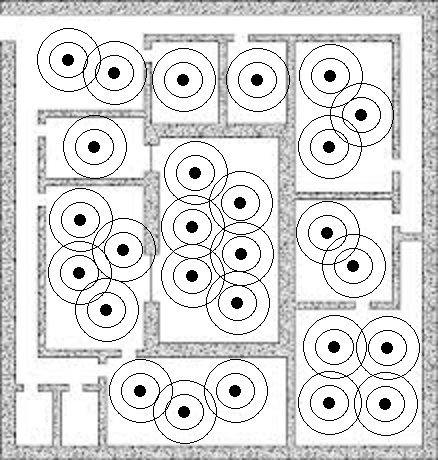
\includegraphics[width=5cm]{images/sensors.jpg}
    \end{figure}
  \end{columns}
\end{frame}

\begin{frame}
  \frametitle{Раскраска графа}
  \begin{columns}[c]
    \column{.5\textwidth}
    Условия:
    \begin{itemize}
      \item каждая вершина может быть раскрашена в один из трех цветов;
      \item смежные вершины должны быть раскрашены в разные цвета.
    \end{itemize}

    \column{.5\textwidth}
    \begin{figure}
       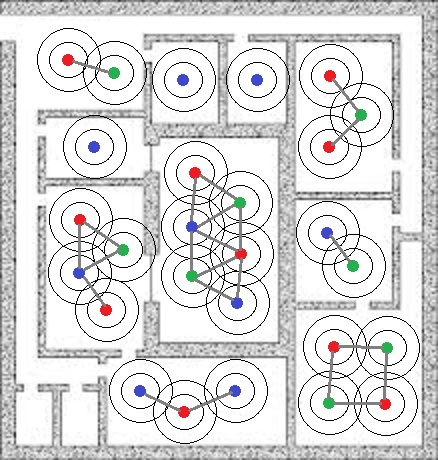
\includegraphics[width=5cm]{images/graph-coloring.jpg}
    \end{figure}
  \end{columns}
\end{frame}

\begin{frame}
  \frametitle{Задачи \alt<5->{оптимизации}{с ограничениями}}
  \alt<6->{\alert{Распределенная задача}}{Задача} \alt<5->{\alert{оптимизации}}{с ограничениями}:
  \begin{itemize}
    \item<1-> множество переменных (сенсор, вершина);
    \item<2-> множества возможных значений для каждой переменной (частота, цвет);
    \item<3-> множество ограничений (перекающиеся сенсоры, смежные вершины);
    \item<5-| alert@6> функция веса для каждого нарушенного ограничения;
    \item<4-> необходимо \alt<5->{\alert{минимизировать сумму весов нарушенных ограничений}}
      {назначить каждой переменной значение, чтобы ограничения были выполнены}.
    \item<6-> распределение переменных по агентам (обычно одна переменная на агента);
  \end{itemize}
  \visible<7->{\alert{Задачи с ограничениями в общем случае NP-полные!}}
\end{frame}

\begin{frame}
  \frametitle{Распределенные задачи}
  Задачи ИИ чаще всего можно сформулировать в виде задачи с ограничениями.

  Подходы к решению:
  \begin{itemize}
    \item адаптация классических решений \\ (перебор, нахождение глобального решения);
    \item адаптация алгоритмов локального поиска \\ (нахождение локального решения);
    \item кооперативные подходы \\ (в основном заимствованные из природы/социологии).
  \end{itemize}
\end{frame}

\begin{frame}
  \frametitle{Асинхронный перебор}
  \begin{figure}
    \includegraphics[width=11cm]<+>{images/ABT/ABT01.png}
    \includegraphics[width=11cm]<+>{images/ABT/ABT02.png}
    \includegraphics[width=11cm]<+>{images/ABT/ABT03.png}
    \includegraphics[width=11cm]<+>{images/ABT/ABT04.png}
    \includegraphics[width=11cm]<+>{images/ABT/ABT05.png}
    \includegraphics[width=11cm]<+>{images/ABT/ABT06.png}
  \end{figure}
\end{frame}

\begin{frame}
  \frametitle{Асинхронный перебор (раскраска графа)}
  \begin{figure}
    \includegraphics[width=10cm]<+>{images/graph-coloring/gc01.png}
    \includegraphics[width=10cm]<+>{images/graph-coloring/gc02.png}
    \includegraphics[width=10cm]<+>{images/graph-coloring/gc03.png}
    \includegraphics[width=10cm]<+>{images/graph-coloring/gc04.png}
    \includegraphics[width=10cm]<+>{images/graph-coloring/gc05.png}
    \includegraphics[width=10cm]<+>{images/graph-coloring/gc06.png}
    \includegraphics[width=10cm]<+>{images/graph-coloring/gc07.png}
    \includegraphics[width=10cm]<+>{images/graph-coloring/gc08.png}
    \includegraphics[width=10cm]<+>{images/graph-coloring/gc09.png}
  \end{figure}
\end{frame}

\begin{frame}
  \frametitle{Асинхронный перебор (ABT)}
  Каждый агент отвечает за одну переменную и предлагает другим агентам принять значение,
  которое он выбрал.
  \begin{itemize}
    \item ABT ~--- полный алгоритм;
    \item глобальное упорядочивание агентов;
    \item нет процедуры останова (но она легко добавляется);
    \item хорошо масштабируется.
  \end{itemize}

  Расширения:
  \begin{itemize}
    \item изменение порядка при конфликтах (AWCS);
    \item решение задачи оптимизации (ADOPT, APO);
    \item динамическое добавление агентов (DynAPO).
  \end{itemize}
\end{frame}

\begin{frame}
  \frametitle{Распределенный локальный поиск}
  Алгоритмы распределенного поиска исследуют возможные изменения состояния:
  \begin{itemize}
    \item всегда стремятся улучшить состояние (уменьшить количество конфликтов);
    \item естественным образом поддерживают динамику (добавление ограничений, агентов);
    \item эффективны по времени;
    \item не полны и требуют настройки параметров.
  \end{itemize}

  Известные алгоритмы:
  \begin{itemize}
    \item Tabu search;
    \item Simulated annealing;
    \item Iterative Breakout method.
  \end{itemize}
\end{frame}

\begin{frame}
  \frametitle{Алгоритмы популяций}
  Популяция ~--- это набор индивидуальных агентов.
  \begin{itemize}
    \item агент знает целиком исходную задачу (и может решить сам);
    \item агенты координируются для нахождения решения.
  \end{itemize}

  Известные алгоритмы:
  \begin{itemize}
    \item эволюционные и генетические алгоритмы;
    \item Particle Swarm Optimization (PSO);
    \item Ant Colony Optimization (ACO).
  \end{itemize}
\end{frame}

\section{Автономность в МАС}

\begin{frame}
  \frametitle{Определение}
  Как и для агента, не существует общепризанного определения автономности:
  \begin{itemize}
    \item автономность ~--- ключевая особенность агентов;
    \item буквально означает <<возможность самоуправления>>.
  \end{itemize}

  В многоагентных системах:
  \begin{itemize}
    \item агент должен проявлять социальную активность и учитывать других участников;
    \item агент должен быть отвественен за свои действия;
    \item баланс между этими требованиями приводит к появлению различных ``уровней автономности''.
  \end{itemize}
\end{frame}

\begin{frame}
  \frametitle{Контролируемая автономность}
  Контролируемая автономность означает способность агентов изменять
  уровень своей (или чужой) автономности:
  \begin{itemize}
    \item это одно из основных средств самоорганизации системы;
    \item делает прозрачным создание адаптивных систем;
  \end{itemize}

  \begin{exampleblock}{}
    {\large ``{\it Контролируемая автономность} ~--- это способность динамически
    обрабатывать внешние воздействия с учётом внутренних мотиваций.''}
    \vskip5mm
    \hspace*\fill{\small--- Bob van der Vecht}
  \end{exampleblock}
\end{frame}

\begin{frame}
  \frametitle{Уровни абстракции при принятии решений}
  Автономность рассматривается в контексте взаимодействия с другими агентами:
  \begin{itemize}
    \item уровень автономности определяет, за какие решения отвечает делегат, а за какие ~--- старший агент;
    \item уровни автономности:
      \begin{itemize}
        \item исполнительный;
        \item планирующий;
        \item целевой;
        \item моральный;
      \end{itemize}
  \end{itemize}
\end{frame}

\begin{frame}
  \frametitle{Социальная автономность}
  Агент может принимать или отказываться от порученных заданий:
  \begin{itemize}
    \item чем менее специфированную задачу может принять агент, тем выше его уровень автономности;
    \item изменение автономности ~--- изменение зависимостей от других агентов;
    \item причины для смены уровня автономности:
      \begin{itemize}
        \item агент не уверен, что может справиться с задачей;
        \item агент предвидит проблемы, которые могут возникнуть;
        \item агент считает, что может лучше справляться с большей автономностью;
        \item агент хочет ``удивить'' старшего сверхурочной работой.
      \end{itemize}
  \end{itemize}
\end{frame}

\begin{frame}
  \frametitle{Возможность и разрешения к действию}
  Автономность определяется свободой выбора и исполнения действий.
  \begin{itemize}
    \item два аспекта: возможность выполнить действие и разрешение на выбор действия;
    \item действия различаются на
      \begin{itemize}
        \item теоретические
        \item практически возможные
        \item возможные (для данного агента)
        \item если возможные действия агента совпадают с ``практически возможными'',
          он считается полностью автономным (по первому аспекту).
      \end{itemize}
  \end{itemize}
\end{frame}

\begin{frame}
  \frametitle{Влияние на групповые решения}
  Автономность измеряется вкладом в групповое решение:
  \begin{itemize}
    \item автономность агента определяется для каждого задания;
    \item уровень автономности определяется степенью независимости
      решения агента от решения любого другого агента.
  \end{itemize}
\end{frame}

\begin{frame}
  \frametitle{Управление процессом принятия решения}
  Агент может передавать управление процессом принятия решения другому агенту или человеку.
  \begin{itemize}
    \item агенты распологают набором стратегий для передачи управления;
    \item агенты могут менять ограничения (например,
      требовать дополнительное время на принятие решения);
    \item временные рамки определяют моменты передачи управления.
  \end{itemize}
\end{frame}

\begin{frame}
  \frametitle{Осознание автономности}
  Важной проблемой является осознание агентом своей автономности:
  \begin{itemize}
    \item осведомлённость о собственной автономности определяет основу ответственности;
    \item предполагается, что агент действует рационально и осознает свой выбор
      с учётом моральных законов;
    \item агент должен осознавать последствия принимаемых решений.
  \end{itemize}
\end{frame}

\section{Применение в адаптивных системах}

\begin{frame}
  \frametitle{Регулирование воздушного траффика}
  Проблемы:
  \begin{itemize}
    \item пилоты коммерческих рейсов вынуждены полагаться на авиадиспетчеров;
    \item чтобы авиадиспетчеры могли справляться со своей задачей, в воздушном
      пространстве ``вычерчиваются'' специальные магистрали;
    \item самолёты регулярно стоят в очередях на такую магистраль;
    \item самолёты на магистрали должны поддерживать установленную скорость,
      чтобы избежать задержек;
    \item со временем растёт потребность в воздушном транспорте и, соответственно,
      увеличиваются задержки.
  \end{itemize}
\end{frame}

\begin{frame}
  \frametitle{Регулирование воздушного траффика}
  Совместное управление воздушным траффиком:
  \begin{itemize}
    \item моделирование воздушного траффика;
    \item агенты ~--- диспетчерские центры (центральный, региональные и каждой авиалинии);
    \item цель ~--- максимально эффективно использовать магистрали.
  \end{itemize}
\end{frame}

\begin{frame}
  \frametitle{Устранение ЧП}
  Пример: авария с возгоранием в туннеле. Вовлечены несколько организаций:
  \begin{itemize}
    \item пожарная бригада;
    \item скорая помощь;
    \item полиция;
    \item администрация;
    \item участники происшествия:
      \begin{itemize}
        \item возможные жертвы;
        \item наблюдатели;
        \item участники дорожного движения.
      \end{itemize}
  \end{itemize}

  Все участники имеют общую цель: устранение ЧП. Обмен информацией важен для корректной
  координации и технологии играют существенную роль.
\end{frame}

\begin{frame}
  \frametitle{Устранение ЧП}
  Пример: авария с возгоранием в туннеле. Вовлечены несколько организаций:
  \begin{itemize}
    \item пожарная бригада;
    \item скорая помощь;
    \item полиция;
    \item администрация;
    \item участники происшествия:
      \begin{itemize}
        \item возможные жертвы;
        \item наблюдатели;
        \item участники дорожного движения.
      \end{itemize}
  \end{itemize}

  Все участники имеют общую цель: устранение ЧП. Обмен информацией важен для корректной
  координации и технологии играют существенную роль.
\end{frame}

\section{Разработка многоагентных систем}

\begin{frame}
  \frametitle{Архитектура агента}
  \begin{itemize}
    \item рассуждающие агенты;
    \item реакционные агенты;
    \item гибридные архитектуры.
  \end{itemize}
\end{frame}

\begin{frame}
  \frametitle{Структуры многоагентной системы}
  \begin{itemize}
    \item организационные шаблоны;
    \item фрактальные системы;
    \item поведенческие паразиты;
  \end{itemize}
\end{frame}

\begin{frame}
  \frametitle{Средства разработки}
  3APL:
  \begin{itemize}
    \item ментальные концепции;
    \item процесс обсуждения;
    \item Prolog-подобный язык для агентов;
    \item Java для программирования действий;
    \item Prolog для программирования убеждений;
    \item сообщения совместимы с FIPA;
    \item последний релиз в 2005 году.
  \end{itemize}
\end{frame}

\begin{frame}
  \frametitle{Средства разработки}
  Jason:
  \begin{itemize}
    \item BDI-модель;
    \item AgentSpeak с расширениями для программирования агентов;
    \item Java для программирования окружения;
    \item KQML и FIPA-ACL для сообщений;
    \item последний релиз в 2009 году.
  \end{itemize}
\end{frame}

\begin{frame}
  \frametitle{Прочие средства}
  Основаны на BDI-модели:
  \begin{itemize}
    \item PRS;
    \item dMARCS;
    \item JACK;
    \item JAM;
    \item Jadex;
    \item Dribble;
    \item Coo-BDI.
  \end{itemize}
\end{frame}

\section{Моя диссертация}

\begin{frame}
  \frametitle{Цели}
  Реализация средств разработки МАС с контролируемой автономностью:
  \begin{itemize}
    \item агенты и окружение должны быть независимы и взаимодействать через
      специфицированный интерфейс;
    \item базовая система должны быть независимой от конкретных архитектур и
      быть достаточно гибкой и расширяемой;
    \item концепции архитектуры агентов и МАС должны быть реализованы в виде библиотеки
      по принципу ``плати за то, чем пользуешься'';
    \item распределенные алгоритмы должны быть доступны в общем виде, готовые к применению
      к частной задаче (не нужно открывать ``велосипед'');
    \item должны быть реализованы различные модели автономности.
  \end{itemize}
\end{frame}

\begin{frame}
  \frametitle{Статус}
  На текущий момент:
  \begin{itemize}
    \item язык реализации ~--- Haskell;
    \item агенты и окружение полностью независимы;
    \item интерфейс представлен набором команд в абстрактном синтаксисе;
    \item абстрактные команды легко экпортируются в другие языки (через C);
    \item код агента с использованием абстрактных команд может быть скомпилирован
      независимо от будущей интерпретации;
    \item общая концепция независит от конкретной архитектуры и легко расширяема;
    \item концепция предусматривает возможность использования <<поведенческих паразитов>>;
  \end{itemize}
\end{frame}

\begin{frame}
  \frametitle{Планы}
  Необходимо реализовать:
  \begin{itemize}
    \item базовые распределенные алгоритмы (ABT, DBA);
    \item базовые ментальные свойства (убеждения, намерения);
    \item базовые модели автономности (социальная, разрешения);
    \item общие средства визуализации МАС;
    \item общие вычислительные среды (многопоточные, распределенные);
    \item FIPA-совместимые сообщения и т.д.
  \end{itemize}

  Кроме того, необходимо продемонстрировать возможности и провести сравнительный анализ
  с существующими средствами разработки.
\end{frame}

\begin{frame}{}
\addtocounter{framenumber}{-1}
\begin{center}
\LARGE{Спасибо за внимание!}
\end{center}
\end{frame}

\end{document}

